\renewcommand{\BrainFuckChapter}{%
  {-}{[}{-}{-}{-}{>}{+}{<}{]}{>}{-}{-}{-}{.}{+}{[}{-}{-}{-}{-}{-}{>}{+}{+}{+}{<}{]}{>}{.}{+}{+}{+}{+}{+}{+}{+}{.}{-}{-}{-}{-}{-}{-}{-}{-}{-}{-}{-}{.}{-}{-}{[}{-}{-}{-}{>}{+}{<}{]}{>}{-}{.}{+}{+}{+}{[}{-}{>}{+}{+}
  {+}{<}{]}{>}{.}{-}{.}{-}{[}{-}{-}{-}{>}{+}{<}{]}{>}{-}{.}{-}{-}{-}{[}{-}{>}{+}{+}{+}{<}{]}{>}{.}{-}{[}{-}{-}{-}{>}{+}{<}{]}{>}{-}{-}{-}{.}{+}{+}{+}{.}{-}{-}{-}{-}{-}{-}{-}{.}{-}{+}{>}{+}{<}{+}{>}{<}{+}{-}{+}{-}
}
\renewcommand{\LifeChapter}{y}

\chapter{Related Work}
\label{ch:related-work}
\section{Traditional Debugging}
\subsection*{Data Dumping}

A common low-tech diagnostic approach is the use of commands that dump
user defined variables to output devices, colloquially referred to as
\emph{printf} commands.
%
On the one hand, such commands are a very powerful tool to both detect
and locate errors.  First, the usage of such commands is normally
pretty straightforward implying a small learning overhead.
%
Also, as the semantics are equal to the ones of the target source
code, its usage is intuitive.
%
Second, as such commands are embedded in the source code, there is no
need for additional tools.
%
Third, as no assumptions are made, it is usable in almost all
imaginable scenarios, being the \textit{de facto} diagnosis fallback
tool.

On the other hand, mostly due to the fact that the usage of dumping
commands is very \textit{ad hoc}, this technique can become
ineffective.
%
First, all dumping commands must be explicitly stated, cluttering the
source code.
%
Second, as all commands must be prepared prior to the application's
execution, a missing print command implies a possible recompilation
and re-execution of the application.
%
Third, with the increase of debugging print commands the amount of
debugging output can become quickly overwhelming.
%
Forth, in order to efficiently use print commands it is required to
have some intuition about the location of the fault.

\subsection*{Debuggers}
In contrast to print commands, debuggers enabled developers to inspect
the internal state of an application without any source code
modifications.

% Post-mortem Debuggers
The first debuggers, referred to as \textit{post-mortem} debuggers,
enabled developers to analyze the status of the registers and memory
after the program's execution.
%
Those tools had however a scalability issue: as the debugger did not
have any information about the source code variables, understanding
the information made available by the debugger was not a trivial task.
%
In order to tackle that problem, symbolic debuggers were developed,
having the capacity of using data generated by the compiler to map
memory addresses onto actual variable names.

% Live Debuggers
\textit{Post-mortem} debuggers were later enhanced with custom
breakpointing features.
%
With custom breakpointing, developers were endowed with the ability of
pausing the program execution at arbitrary locations, analyzing its
status and finally resuming its execution.
%
The final breakpoint related improvement was the introduction of
conditional breakpoints.
%
This feature enables developers to pause the program's execution based
on arbitrary rules.
%
A well known example of a debugger is \emph{GNU}'s \emph{GDB}
\citep{Stallman02}.


\section{Software Testing}

\subsection*{Assertions/Oracles}
Assertions/oracles are mechanisms that check for invariant violations
at run-time \citep{Rosenblum95}.
%
Whenever an invariant is broken, the application's execution is
halted.
%
This behavior, on the one hand, prevents an error state from
propagating to other components and, on the other hand, reduces the
scope of search for errors.
%
In contrast to dumping commands, with the increase in the number of
assertions, the diagnosis of errors becomes easier.
%
Despite implying a performance penalty in the target application,
assertions can normally be disabled and thereby not included in
release versions of the applications.

Assertions can be broadly divided in two groups: \emph{pre-conditions}
and \emph{post-conditions}.
%
Pre-conditions check for the validity of the inputs to a particular
component.
%
Post-conditions check whether or not the component
performed as expected (\ie, the validity of the output).
%
While pre-conditions are often easy to define, its normally hard to
define a ``good'' validity test for the output.
%
We quoted good due to the fact that the meaning of ``good'' is context
dependent.
%
In fact, the quality of an assertion is normally a trade-off between
correctness and complexity.

As an example consider the ``quicksort'' sorting algorithm ($\bigO{n \cdot
  log(n)}$ complexity).
%
A simple postcondition would be that the size of the output matches
the size of the input ($\bigO{1}$ complexity).
%
This condition is able to detect outputs with wrong sizes, but fails
to detect unsorted outputs.
%
A more robust postcondition would be to check that $\forall_{A_n}: A_n
>= A_{n - 1}$ ($\bigO{n}$ complexity).
%
This condition is able to detect unsorted outputs, but fails to detect
outputs that have elements that are not present in the input.
%
An even more robust post-condition would be to compute the output with
a different algorithm or implementation and compare it with the output
under test ($\bigO{n\cdot log(n)}$).


Oracles can also be used to assure dependability at run-time by
implementing \ac{TMR} \citep{Lyons62,Johnson10}.
%
\ac{TMR} is a form of \emph{N-modular} redundancy in which three
components perform the same task and the system's output is determined
by a majority-voting process, producing a single output.
%
A \ac{TMR} system not only increases the likelihood of detecting
errors but also opens the possibility of masking errors in the event
of a minority of the redundant components performing erroneously.


In order to automate the process of creating assertions, approaches
that automatically detect invariants (\eg, range) in arbitrary system
variables (known as fault screeners) were proposed
\citep{Abreu08c,Ernst00,Ernst01,Ernst07,Hangal02,Pinto15,Racunas07}.

\subsection*{Test Suites}
\label{sec:related-work:testing}
Test suites are collections of tests cases aimed automatically
validating the functional requirements of systems \citep{Huizinga07}.
%
Test suites are normally composed of unit tests, \ie, smaller tests
that are focused on testing a particular functionality of the system
in isolation.

In order to ease the creation of unit tests, a vast set of unit
testing frameworks for several languages have been proposed.
%
Well-known unit testing frameworks include:
\begin{itemize}[nolistsep]
\item \emph{Check}\footnote{\url{http://check.sourceforge.net/}} for \emph{C}.
\item \emph{Boost}'s Unit Test
  Framework\footnote{\url{http://www.boost.org/doc/libs/release/libs/test/}}
  for \emph{C++}.
\item \emph{JUnit}\footnote{\url{http://junit.org/}} for \emph{Java}.
\item \emph{unittest}\footnote{\url{https://docs.python.org/3/library/unittest.html}} for
  \emph{Python}.
\end{itemize}

While test suites are normally manually created, they are often the
basis of a large number of automatic techniques.
%
For instance, in the scope of software testing, regression testing
\citep{Vokolos98} enables developers to easily uncover eventual faults
introduced by changes made to a base version of some software by
automatically running an appropriate test suite on the new version of
the software.

Even though regression testing contributes to a higher software
quality, it may become cost ineffective due to several reasons.
%
First, if the test suite has a low fidelity, \ie, a low capacity for
correctly detecting errors, the resources needed to use it may not
justify the marginal reliability improvement.
%
Second, if a software grows to a fair size, the time needed to test it
may become impractical.
%
Third, a test suite may easily contain test redundancy leading to
resource waste.

To mitigate the problem of low fidelity test suites, the concept of
mutation analysis was introduced \citep{DeMillo78}.
%
Mutation analysis works by iteratively injecting the system with one
artificial bug and then executing the test suite.
%
If the injected fault goes undetected, it shows a case where the test
suite potentially fails to detect an error and therefore needs
improvement.
%
On the one hand, mutation analysis methods evaluate how good a test
suite is at uncovering faults and, on the other hand, give insight
into how and where a test suite needs improvement.
%
Mutation analysis is also used as a way of automatically generating
test cases \citep{Fraser11,Fraser12,Fraser13,Campos13b}.
%

To reduce amount of testing needed, methods for prioritizing a test
suite (test case prioritization) have been developed
\citep{Rothermel99,
  Rothermel01,Bryce07,Sanchez11,Elbaum02,Sun13,Huang10}.
%
Such approaches determine an execution order for the test cases such
that the first tests to be executed are the ones that have the best
chance to uncover errors.
%
With a prioritized test suite it is possible to more efficiently test
a software.

To maintain a test suite over time it is necessary to remove
redundancies/inconsistencies.
%
A similar problem in terms of concept is the problem of selecting a
subset of the test suite that satisfies a set of constraints while
maximizing/minimizing a particular score (\eg, code coverage and/or
oracle cost).
%
This problem is referred to as the test suite minimization problem.
%
In order to tackle test case minimization problem, automatic solutions
that use constraint solvers have been proposed
\citep{Arito12,Campos13a,Mondal15}.
%
It is important to note, however, that the reduction in the test suite
size may have a negative impact in its fault detection capabilities
\citep{Rothermel98}.



\section{Instrumentation}
\subsection*{Code Instrumentation}
In order to obtain information about a system during its execution, it
needs to be injected with instrumentation code that captures the
desired data \citep{Garlan95}.
%
Instrumentation code normally relies on a series of \emph{trampolines}
to an arbitrary function \texttt{foo()} that deals with the specifics
of the data collection
(\Cref{fig:related-work:instrumentation-program}).
%


\begin{figure}[ht]
  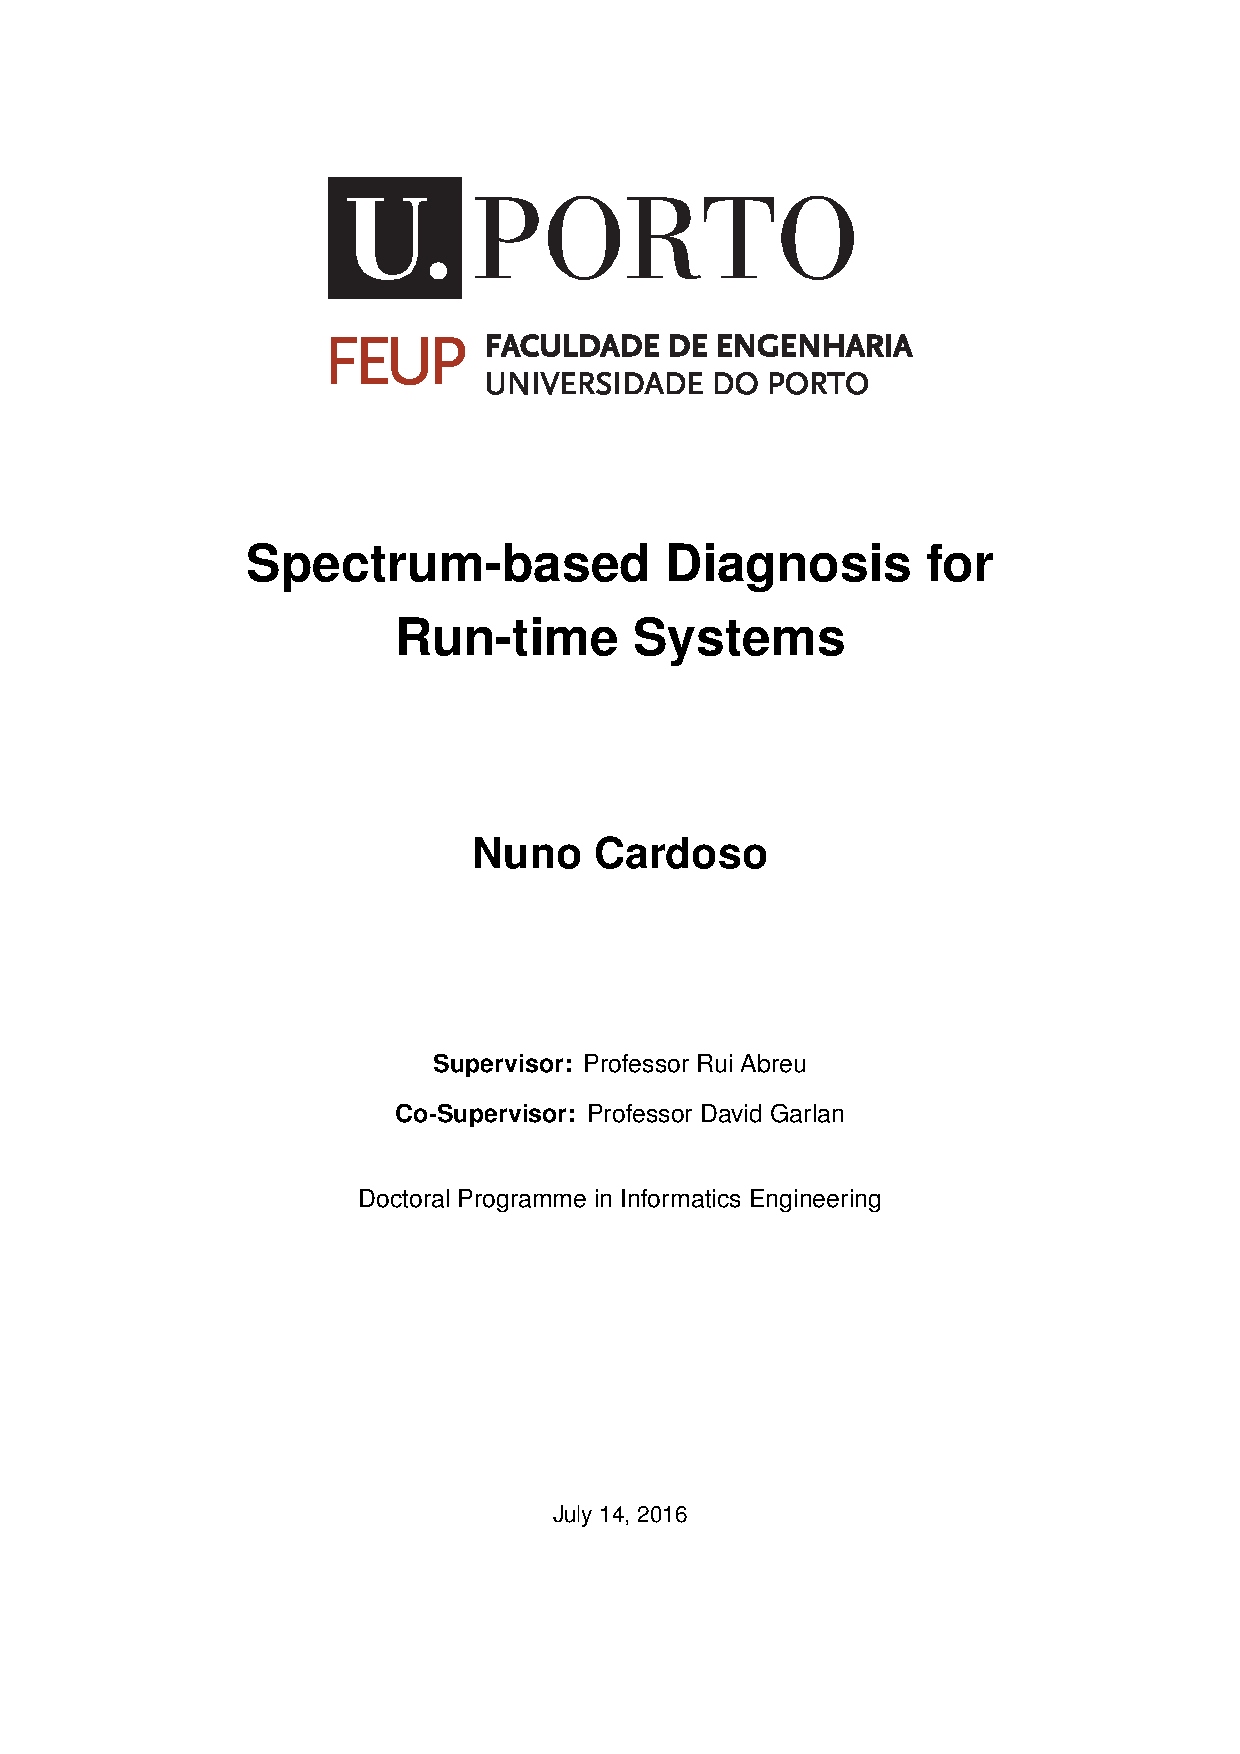
\includegraphics[width=0.9\columnwidth,page=1]{figures/related_work/figures/main.pdf}
  \caption{Instrumentation code insertion (adapted from \citep{Tikir02})}
  \label{fig:related-work:instrumentation-program}
\end{figure}


Instrumentation is used in a wide diversity of domains.
%
In addition to most of the techniques presented in this chapter and in
this thesis, instrumentation is used in \citep{Kumar05}:
\begin{itemize}[nolistsep]
\item Demand-driven structural software testing \citep{Misurda05}.
\item Dynamic optimizers \citep{Arnold01,Hong15,Bala00}.
\item Modeling computer architecture features \citep{Cmelik95,Scott03,Witchel96}.
\item Software security \citep{Kiriansky02,Scott02,Song08}.
\end{itemize}

Several instrumentation techniques have been proposed.
%
These techniques include:
\begin{itemize}[nolistsep]
\item Manually placing instrumentation in a program before it
  executes.
\item Static binary modification \citep{Bus04,Larus95,Srivastava94}.
\item Dynamic/Live instrumentation in executing programs
  \citep{Arnold01,Hollingsworth97,Luk05a,Luk05b,Lattner02,Nethercote03}.
\end{itemize}




\subsection*{Code Coverage}
\label{sec:related-work:code-coverage}
Code coverage is an analysis method that determines which parts of a
particular system have been executed (covered) during a test run
\citep{Miller63,Graham06}.
%
Well known examples of code coverage tools are
\emph{EMMA}\footnote{\url{http://emma.sourceforge.net/}} and
\emph{Cobertura}\footnote{\url{https://cobertura.github.io/cobertura/}}
(see \citep{Yang06} for more examples).





In the scope of \ac{SFL}, by using a code coverage tool in conjunction
with a test suite, it is possible to create spectra and thereby
identify which components are more likely to be involved in the test
suite failure.
%
To solve the potential scalability issues that \ac{SFL} techniques may
have when instrumenting large software programs, a dynamic
instrumentation approach, called \ac{DCC}, was proposed
\citep{Perez12a}.
%
This technique automatically adjusts the instrumentation granularity
of the system under analysis.
%
First, the system is instrumented using a coarse granularity (\eg,
package level in \emph{Java}).
%
Then, \ac{SFL} is executed and, based on the diagnostic results,
\ac{DCC} decides which components should be re-instrumented with a
finer granularity level (\eg, in \emph{Java} one should instrument
classes, then methods, and finally statements).
%
After re-instrumenting the selected components, the tests that
activate the re-instrumented components are re-executed.
%
This loop is repeated until \ac{SFL} yields an useful diagnostic
report.

\ac{DCC}, as an iterative technique, is aimed at improving the
execution time of the fault localization procedure, and shows a
substantial reduction of the execution time ($27\%$ on average) and
the diagnostic report size ($67\%$ on average), when compared to
normal \ac{SFL} executions \citep{Perez12a}.
%
However, for small projects, the overhead of re-instrumenting and
re-running tests may consume more time than performing a single
iteration with a fine-grained instrumentation throughout the entire
project.
%
To prevent this, an approach that uses a lightweight topology model of
the system to decide whether or not \ac{DCC} should be used was
proposed \citep{Perez12b}.

Code coverage is also used in the scope of \ac{GUI} testing as an aid
in determining whether a \ac{GUI} has been adequately tested
\citep{Memon01}.
%

\subsection*{Profilers}
\label{sec:related-work:profiling}

Profiling is a dynamic analysis that gathers some metrics from the
execution of a system, such as memory usage and frequency/duration of
component activations.
%
Even though the main use of profilers is in system optimization
processes, it is also useful for debugging purposes, such as:

\begin{itemize}[nolistsep]
\item Knowing if components are being called more or less often than
  expected.
\item Finding if certain components execute slower than expected or if
  they contain memory leaks.
\item Investigating the behavior of lazy evaluation strategies.
\end{itemize}

Well known profiling tools include \emph{GNU}'s \emph{gprof}
\citep{Graham82}, \emph{Valgrind} \citep{Nethercote03}, and
\emph{Java's VisualVM}\footnote{\url{http://visualvm.java.net/}}.



\subsection*{Run-time Spectra Collection}
Research on \ac{SFL} has been mostly targeted at development-time
environments.
%
In such environments, the spectrum is normally used to diagnose errors
occurring during the execution of a test suite.
%
The availability of a test suite enables a simple approach to collect
spectra due to the fact that every single unit test corresponds to a
transaction in the spectrum abstraction.
%
Also, as the purpose of a test suite is to evaluate the correctness of
a program with regard to a specification, the error information is
also ``freely'' available.
%
Furthermore, due to the fact that unit tests normally target a set of
tightly coupled components (normally contained within a single
process) it is possible to perform a direct monitoring by injecting a
code-level instrumentation.

In contrast to development-time, in run-time environments the process
of obtaining the spectra required to perform diagnosis is much more
complex due to several aspects.
%
First, performing active (and controlled) tests (\eg, unit tests) on
deployed systems is normally not possible without disrupting their
services.
%
The impossibility of using controlled tests to evaluate the
correctness of the system, forces the spectra collection mechanisms to
rely on coarse grained invariants (\eg, response time, memory usage,
\etc) to assert the validity of a set of components' activation.
%
This is normally accomplished by encoding such constraints using an
\ac{ADL} (\eg, \citep{Garlan00}).

Second, as the concept of transaction is system-dependent, some
mechanism must be used to relate component activity with transactions.
%
A common approach is to use an \ac{ADL} specification of the system in
which the relevant communication paths between components are defined
and, the activation of such paths, generates transactions.
%
In \citep{Casanova11}, the authors use a form of message sequence
charts to define the relevant computations and how they relate to form
transactions.
%
In \citep{Casanova13}, the authors propose an \ac{ADL} that
features a set of constructs that enable the encoding of rules
describing transaction types.
%
In order to ease the definition of the rules, this \ac{ADL} makes use
of object oriented concepts such as inheritance, enabling model reuse
and refinement.
%
In \citep{Piel12}, the authors divide the system execution in
transactions by setting an arbitrary transaction frequency.
%
This approach requires that an appropriate frequency value is
defined in order to produce useful spectra.
%
On the one hand, if the frequency is too low,
transactions that activate almost all components will be
created\footnote{The consequence of activating all components is that
  the resulting spectra has low entropy which, in practice, results in
  a low quality diagnosis.}.
%
On the other hand, if the frequency is too high, the components
that triggered failures may not be contained in any of the failing
transactions.
%
In order to reduce the sensitivity of the approach with regard to the
frequency parameter, the authors propose that an exponential
distribution (with average equal to the target frequency) is used to
generate random transaction durations.

Third, most systems operate continuously raising the challenge of
determining which transactions are of interest for diagnostic
purposes.
%
In contrast to development-time, in a run-time environment the
observations may age with time and reflect old states of the system
(\eg, having a failing transaction in the spectra caused by an
already fixed problem) and hamper the diagnosis quality.
%
On the one hand, if all the available spectra are used, it is possible
that outdated information may degrade the diagnosis system
performance.
%
On the other hand, if too few transactions are used, the diagnosis
system may not be able to isolate the correct candidate.
%
In \citep{Casanova13}, the authors discard the spectra every time a
correction is made on the system and collect spectra until the entropy
in the diagnosis report is below an arbitrary threshold.
%
The entropy is used to characterize the (im)purity of a ranking of
diagnosis candidates.
%
The idea is to adapt the time window considering the entropy, knowing
that a larger spectrum normally decreases the entropy of the ranking.
%
In \citep{Piel12}, the authors use a time-based sliding window at the
end of which the transactions are discarded.
%

Fourth, most systems do not provide monitoring interfaces.
%
In \citep{Casanova13}, the authors instrument the system by
intercepting operating system calls (\eg, bind, accept, socket, \etc)
which are then translated and fed to the rule system.



\section{Automated Diagnosis}
\subsection*{Delta Debugging}
\emph{Delta Debugging} is a technique that tries to systematically
simplify the input that leads a certain system to a failure
\citep{Zeller02a}.
%
This is accomplished by iteratively reducing the size of the input
until the smallest input that causes the execution to fail is reached
\citep{Zeller02b,Cleve05}.
%
This is done under the assumption that that simpler inputs activates
less components than more complex inputs and, therefore, renders the
system easier to debug.


\begin{figure}[!ht]
  \bgroup
  \def\x{{\Large$\bullet$}}
  \begin{tabular}{c|cccccccc|c}
    Input & $1$ & $2$ & $3$ & $4$ & $5$ & $6$ & $7$ & $8$ & Error \\ \hline
    $1$   & \x  & \x  & \x  & \x  & \x  & \x  & \x  & \x  & $1$   \\
    $2$   & \x  & \x  & \x  & \x  & .   & .   & .   & .   & $?$   \\
    $3$   & .   & .   & .   & .   & \x  & \x  & \x  & \x  & $1$   \\
    $4$   & .   & .   & .   & .   & \x  & \x  & .   & .   & $0$   \\
    $5$   & .   & .   & .   & .   & .   & .   & \x  & \x  & $1$   \\
    $6$   & .   & .   & .   & .   & .   & .   & \x  & .   & $1$   \\
    $7$   & .   & .   & .   & .   & .   & .   & .   & \x  & $0$   \\
  \end{tabular}
  \egroup
  \caption{Delta debugging example (adapted from \citep{Zeller02a} and
    \citep{Perez14a})\label{fig:related-work:dd-example}}
\end{figure}

Consider the example in \Cref{fig:related-work:dd-example}, in which a
system takes as input a set of integers in the interval $[1,8]$.
%
Initially, the system is executed with an input consisting of all
possible elements in the input space (input $1$ in the figure).
%
As this input makes the system fail, the next step is to split the
input, as is the case in inputs $2$ and $3$.
%
It is important to note that, when manipulating the system's input,
one can reach one of three possible outcomes: passed ($0$), failed
($1$), and unresolved ($?$).
%
The latter occurs when the system receives an invalid input.

The next steps of the delta debugging algorithm are to keep attempting
to reduce the size of the failure inducing inputs.
%
In this example, input $3$ is divided into inputs $4$ and $5$, and, in
turn, input $5$ is divided into inputs $6$ and $7$.
%
As can be seen in the figure, input $6$ is a minimal failure inducing
input.

Since a vast amount of combinations may result in passed/unresolved
outcomes, in \citep{Misherghi06}, the authors propose an improved
algorithm, called \emph{Hierarchical Delta Debugging}.
%
This technique takes into account the input structure to reduce the
number of inputs to examine.
%
By initially using a coarser level of detail, the algorithm is able to
prune large irrelevant portions of the input early in the minimization
process.
%
Besides speeding up the delta debugging process, the hierarchical
technique also has the advantage of producing better (and more easily
understandable) diagnostic reports, as the output is a structured tree
\citep{Perez14a}.
%


\subsection*{Static/Dynamic Slicing}
\emph{Static Slicing} \citep{Weiser82,Weiser84} is a debugging
approach that starts from the failure and uses the control and data
flow of the system as a backwards reasoning method to narrow down the
set of potential faulty components.
%
This is accomplished by ignoring all components that have no data or
control dependencies to the variables used in the error detection
process.
%
In this context, a \emph{slice} is a subset of the system's components
that directly or indirectly influences the values of a given set of
state variables.
%

A problem of static slicing is that the slices computed by means of
static analysis tend to be large.
%
In \citep{Lyle87}, the authors were able to reduce the slices' size by
constructing \emph{dices}.
%
A \emph{dice} is the set difference between two static slices of a
system.
%
To further decrease the slices' size, in \citep{Kolettis95}, the
authors propose an approach, called \emph{Dynamic Slicing}, that
relies on execution information to determine which components belong
to the slice (or dice).

Dynamic slices occasionally omit components responsible for the
system's failures.
%
To mitigate this problem, in \citep{Zhang04,Zhang05,Zhang07}, the
authors introduced the concepts of dynamic dependence graph, implicit
dependencies and relevant slicing, in \citep{Agrawal95}, the authors
propose the usage of execution slices and, in \citep{Wong06}, the
usage of inter-block data dependencies.

In \citep{Wotawa10}, the authors improve dynamic slicing by combining
it with \ac{MBD} techniques.
%
In \citep{Hofer12}, the authors show that the aforementioned can be
further improved by combining it with \ac{SFL}.
%
In \citep{Xie10,Xie13}, the authors introduce the concept of
metamorphic slice with the goal of enabling the usage of \ac{SFL}
without the need for test oracles.


\subsection*{Similarity-based \acs{SFL}}
\label{sec:related-work:similarity-based-SFL}
An alternative approach to \ac{SFL} is to use similarity coefficients
as a way of determining which columns of matrix $A$ resemble the most
with the error vector $e$ the most or, in other words, which
components have the activity pattern most similar to the error
pattern.
%
The underlying assumption of this approach is that a component with an
activation pattern resembling the error pattern is likely to be at
fault.

Similarity coefficient-based approaches are known for being extremely
lightweight at the cost of only being capable of proposing single
component candidates.
%
Given that the candidate generation problem is implicitly solved by
making such assumption, all $M$ components (\ie, all the single fault
candidates) are ranked according to their similarity scores.


Several similarity coefficients do exist \citep{Abreu09a}.
%
Well known examples include the \emph{Jaccard} coefficient
$\fn{s_J}$ used in the \emph{Pinpoint} tool~\citep{Chen02}, the
$\fn{s_A}$ coefficient used by the \emph{AMPLE} tool
\citep{Dallmeier05} and the $\fn{s_T}$ coefficient used in the
\emph{Tarantula} tool \citep{Jones05}:

\begin{equation}
  \label{eq:related-work:jaccard}
  \fn{s_J}(j) = \frac{\nfunc{11}}{\nfunc{11}+\nfunc{01}+\nfunc{10}}
\end{equation}

\begin{equation}
  \fn{s_A} (j) = \bigg| \frac{\nfunc{11}}{\nfunc{01}+\nfunc{11}} - \frac{\nfunc{10}}{\nfunc{00}+\nfunc{10}} \bigg|
\end{equation}

\begin{equation}
  \label{eq:related-work:tarantula}
  \fn{s_T}(j) = \frac{\frac{\nfunc{11}}{\nfunc{11}+\nfunc{01}}}{ \frac{\nfunc{11}}{\nfunc{11}+\nfunc{01}} + \frac{\nfunc{10}}{\nfunc{10}+\nfunc{00}}}
\end{equation}

\noindent where:
%
\begin{itemize}[nolistsep]
\item $\nfunc{11}$ is the number of failed runs in which component $j$ is involved.
\item $\nfunc{10}$ is the number of passed runs in which component $j$ is involved.
\item $\nfunc{01}$ is the number of failed runs in which component $j$ is not involved.
\item $\nfunc{00}$ is the number of passed runs in which component $j$ is not involved.
\end{itemize}

Formally, $n_{pq}$ is defined as:
\begin{equation}
  \label{eq:related-work:occurrence}
  \nfunc{pq} = |\set{i\mid A_{ij}=p \wedge e_i=q}|
\end{equation}


One of the best performing similarity coefficients for fault
localization is the \emph{Ochiai} coefficient \citep{Abreu07}.
%
The \emph{Zoltar} \citep{Janssen09} and \emph{GZoltar}
\citep{Campos12} fault localization tools use the \emph{Ochiai}
coefficient to quantify the resemblance between components' activity
and the error vector.
%
This coefficient was initially used in the molecular biology
domain~\citep{Meyer04}, and is defined as follows:

\begin{equation}
  \label{eq:related-work:ochiai}
  \fn{s_O}(j) = \frac{\nfunc{11}}{\sqrt{\big(\nfunc{11}+\nfunc{01}\big)\cdot\big(\nfunc{11}+\nfunc{10}\big)}}
\end{equation}
\noindent

It is important to note, however, that, even though similarity scores
range between $0$ and $1$, they are not considered to be
probabilities \citep{Li13}.
%
In fact, the \emph{Ochiai} coefficient corresponds to the the cosine
of the angle between $2$ vectors in a $n$-dimensional space.


Due to its good performance at an extremely low cost, similarity-based
\ac{SFL} has already been applied in a variety of domains:
\begin{itemize}[nolistsep]
\item In \citep{Hofer13}, the authors compare the techniques presented
  in \citep{Wotawa10} (Spectrum-enhanced Dynamic Slicing),
  \citep{Abreu09f} (\ac{SFL}), and \citep{Abreu12} (Constraint-based
  Debugging) when applied in spreadsheet debugging.
  %
  Promising results were observed for both spectrum-based approaches.
\item In \citep{Abreu14}, the authors use \ac{SFL} together with
  spreadsheets smells \citep{Cunha12a,Cunha12b,Hermans12a,Hermans12b}
  to detect and diagnose problems in spreadsheets.
\item In \citep{Machado13}, the authors use \ac{SFL} for debugging
  mobile applications.
\item In \citep{Passos14,Passos15}, the authors apply \ac{SFL} in the
  scope of multi-agent systems.
\item In \citep{Zoeteweij07}, the authors apply \ac{SFL} in the scope of
  embedded systems.
\item In \citep{Perez14b}, the authors use \ac{SFL} for software
  comprehension.
\end{itemize}

\subsection*{Candidate Generation}
In \citep{Reiter87}, the authors propose a breadth-first search
algorithm to solve the \ac{MHS} problem.
%
Later, in \citep{Wotawa01,Greiner89}, some improvements over the base
algorithm have been suggested.

In \citep{Zhao07} a method using set-enumeration trees to derive all
\acp{MHS} in the context of model-based diagnosis is presented.
%
While sound and complete, such algorithms do not scale to large
problems.
%
To overcome this problem, in \citep{Feldman08}, the authors propose a
stochastic search algorithm, that starts with a \ac{HS} $d$ for
$(U, S)$ and iteratively removes elements from $d$ while guaranteeing
that the resulting set still is a $\ac{HS}$.
%
By using a stochastic search, the algorithm trades-off
soundness/completeness for computational efficiency.

In contrast to our approach, all of the above algorithms make use of a
constraint solver to check whether or not a set $d$ is a \ac{HS}.
%
On the one hand, such approaches do not require an explicit
availability of set $S$, making them useful for scenarios where the
problem is not explicitly stated but rather indirectly observed.
%
On the other hand, as a great part of the ``heavy-lifting'' is
performed by third-party libraries, their performance is largely
limited by the performance of the underlying constraint solver.
%
Furthermore, and contrary to our work, the mentioned algorithms do not
use any other information aside from the problem statement $(U,S)$
(recall that our heuristic is arbitrary and can use information
outside of the problem statement).


In \citep{Fijany04,Fijany05}, the \ac{MHS} problem is mapped onto an
$1/0$-integer programming problem.
%
Contrary to our work, this approach does not use any other information
aside from the problem statement $(U,S)$.

In \citep{Vinterbo00,Li02,Aickelin04,Huang94}, several genetic algorithms
to compute \acp{MHS} are proposed.
%
While scalable to large problems, these algorithms do not guarantee
soundness nor completeness.

\subsection*{Visualizations}
Several authors acknowledged the fact that humans have difficulties in
interpreting a diagnostic report as presented in
\CrefPageParen{def:intro:diagnostic-report} \citep{Jones04}.
%
To improve the user-friendliness and thereby the utility of automated
diagnostic tools, several visual approaches were proposed:
\begin{itemize}[nolistsep]
  %
\item In \citep{Jones02,Jones05}, the authors present a technique that
  uses color to visually map the participation of each component in
  the outcome of the execution of the program with a test suite.
  %
\item In \citep{Orso04}, the authors propose a generalization of
  approach presented in \citep{Jones02} that enables a color-based
  representation of bi-dimensional component data by both using the
  hue and the brightness values.
  %
\item In \citep{Bouillon07}, the authors present a color coded
  call-graph in which the same color code is used.
  %
\item In \citep{Janssen09}, the authors present a tool that colors
  each line in the application's source code according to its
  \ac{SFL} score.
  %
\item In \citep{Campos12}, the authors improve the tool by adding
  two visualizations: \emph{Treemap} and \emph{Sunburst}
  \citep{Riboira11}.
  %
\item In \citep{Gouveia13}, the authors re-implement the same
  visualizations using \emph{HTML5} to improve the tool's portability.
\end{itemize}
